% -*- TeX:de -*-
\NeedsTeXFormat{LaTeX2e}
\documentclass[12pt,a4paper]{article}
\usepackage[german]{babel} % german text
\usepackage[DIV12]{typearea} % size of printable area
\usepackage[T1]{fontenc} % font encoding
%\usepackage[latin1]{inputenc} % most likely on Windows
\usepackage[utf8]{inputenc} % probably on Linux
\usepackage{multicol}

% PLOTTING
\usepackage{pgfplots} 
\usepackage{pgfplotstable}
\usepackage{url}
\usepackage{graphicx} % to include images
\usepackage{tikz}
\usepackage{subfigure} % for creating subfigures
\usepackage{amsmath} % a bunch of symbols
\usepackage{amssymb} % even more symbols
\usepackage{booktabs} % pretty tables
\usepackage{makecell} % multi row table heading

% a floating environment for circuits
\usepackage{float}
\usepackage{caption}

%\newfloat{circuit}{tbph}{circuits}
%\floatname{circuit}{Schaltplan}

% a floating environment for diagrams
%\newfloat{diagram}{tbph}{diagrams}
%\floatname{diagram}{Diagramm}

\selectlanguage{german} % use german

\begin{document}

%%%%%%% DECKBLATT %%%%%%%
\thispagestyle{empty}
			\begin{center}
			\Large{Fakultät für Physik}\\
			\end{center}
\begin{verbatim}


\end{verbatim}
							%Eintrag des Wintersemesters
			\begin{center}
			\textbf{\LARGE SS 14}
			\end{center}
\begin{verbatim}


\end{verbatim}
			\begin{center}
			\textbf{\LARGE{Physikalisches Praktikum\\ für das Bachelorstudium}}
			\end{center}
\begin{verbatim}




\end{verbatim}

			\begin{center}
			\textbf{\LARGE{PROTOKOLL}}
			\end{center}
			
\begin{verbatim}

\end{verbatim}

			\begin{flushleft}
			\textbf{\Large{Experiment (Nr., Titel): PS10 - Wärmeleitung in Metallen und Isolatoren, Spezifische Wärmekapazität von Metallen}}\\
							%Experiment Nr. und Titel statt den Punkten eintragen
			\LARGE{PS09 }	
			\end{flushleft}

\begin{verbatim}

\end{verbatim}	
							%Eintragen des Abgabedatums, oder des Erstelldatums des Protokolls
			\begin{flushleft}
			\textbf{\Large{Datum:}} \Large{08.05.2014}
			\end{flushleft}
			
\begin{verbatim}
\end{verbatim}
							%Namen der Protokollschreiber
		\begin{flushleft}
			\textbf{\Large{Namen:}} \Large{Patrick Braun, Johannes Kurz}
			\end{flushleft}

\begin{verbatim}


\end{verbatim}
							%Kurstag und Gruppennummer, zb. Fr/5
			\begin{flushleft}
			\textbf{\Large{Kurstag/Gruppe:}} \Large{DO/4}
			\end{flushleft}

\begin{verbatim}

\end{verbatim}
							%Name des Betreuers, das Praktikum betreute.
			\begin{flushleft}
			\LARGE{\textbf{Betreuer:}}	\Large{Johanna Akbarzadeh}	
			\end{flushleft}

%%%%%%% DECKBLATT ENDE %%%%%%%
\pagebreak
\setlength{\columnsep}{20pt}
\begin{multicols}{2}

%%%%%%%%%%%%%%%%%%%%%%%%%%%%%%%%%%%%%%%%%%%%%%%%

%\begin{figure}[H]
%	\centering
%	\includegraphics[scale=0.35]{./data/beugung.png}
%	\caption{Beugungsmuster Einzelspalt (echtes Foto; schwarz durch weiß ersetzt)}
%	\label{fig:beugungsmuster}
%\end{figure}


%\begin{figure}[H]
%	\centering
%	\pgfplotstabletypeset[
%			columns={abstand, n},
%			col sep=&,
%			columns/abstand/.style={precision=2, zerofill, column name=\makecell{$Abstand$\\$(\pm 0.05)[mm]$} }, 
%			columns/n/.style={column name=\makecell{$n$\\$(Ordnung)$}, precision=0},
%			every head row/.style={before row=\hline,after row=\hline\hline},
%			every last row/.style={after row=\hline},
%			every first column/.style={column type/.add={|}{} },
%			every last column/.style={column type/.add={}{|} }
%			]{
%			abstand & n
%			12.9 & 1
%			24.45 & 2
%			37.40 & 3
%			49.35& 4
%			62.45 & 5
%			74.45 & 6
%			87.45 & 7
%			100.25 & 8
%			
%			}
%	\caption{Messwerte Einzelspalt}
%	\label{tab:werte_einzelspalt}
%\end{figure}


%%%%%%%%%%%%%%%%%%%%%%%%%%%%%%%%%%%%%%%%%%%%%%%%
%%%%%%%%%%%%%%%%%%%%%%%%%%%%%%%%%%%%%%%%%%%%%%%%
\noindent In den folgenden Experimenten bestimmen wir die Transporteigenschaften von Festkörpern in Bezug auf Wärme. Kennzahlen die sich im laufe der Geschichte heraus kristallisiert haben sind:\\
\begin{itemize}
	\item Temperaturleitfähigkeit
	\item Wärmeleitfähigkeit
\end{itemize}
Diese geben an wie gut (oder schlecht bei Isolatoren) Temperaturen und somit Wärme im Festkörper propagiert werden.

\section{Wärmeleitfähigkeit von Metallen - thermografische Bestimmung}

\subsection{Grundlagen}
Um die Temperaturleitzahl zu errechnen wird die Wärmeleitungsgleichung für den eindimensionalen Fall gelöst ([1] p.8). Dabei ergibt sich der Faktor 
$$\chi = \frac{\lambda}{\rho*c}$$
Nach dem Übergang zum Zielmedium ([1] p. 8 Abb. 2) kann das Temperaturprofil unter zur Hilfenahme der Gauss'schen  Fehlerfunktion folgend beschrieben werden
$$T(x,t) = (T_0 - T_{max}) * $$
$$ * erf(\frac{1}{\sqrt{4 * \chi * t}})+T_{max}$$
Über einen nicht-linearen Fit der Form $(A-B) * erf(C * x) + B$ kann aus den Messdaten der Faktor C ausgedrückt werden.
Dadurch erhalten wir die Temperaturleitfähigkeit $\chi$ bzw. die Wärmeleitfähigkeit $\lambda$ zu einem bestimmten Zeitpunkt t:
$$\chi = \frac{1}{c^2 * 4 * t}$$
$$\lambda = \chi * \rho * c$$
wobei $\rho = (7480 \pm 350)\frac{kg}{m^3}$\\ 
und $c_{32^{\circ}C} = (454.6 \pm 0.7)\frac{J}{kg * K}$\\
\\
Bei einem konstanten Wärmestrom
$$\phi = const.$$
kann näherungsweise die Lösung ([1] p. 9 Glg. 8) 
$$\frac{\Delta Q}{\Delta t} = -\lambda * A * \frac{dT}{dx}$$
verwendet werden.
Hierbei wird der Wärmestrom durch die Quelle konstant gehalten. Darüber hinaus kann $\frac{dT}{dx}$ über die Steigung eines linearen Fit approximiert werden.
Die Fläche der Probe kann gemessen werden. Durch einfaches umformen ergibt sich für die Wärmeleitfähigkeit:
$$ \lambda = - \frac{\Delta Q}{\Delta t} * \frac{1}{A * \frac{dT}{dx}} $$
\subsection{Versuchsaufbau}
Der erste Versuch gliedert sich in zwei Teilgebiete. Im ersten Teilgebiet betrachten wir zwei Metallstäbe (Eisen, lackiert). Einer der beiden wird auf 40 Grad erwärmt und der andere verbleibt bei Raumtemperatur. Mit ein wenig Wärmeleitpaste werden beide Stäbe zusammengefügt und mit der Wärmebildkamera (Abb. \ref{}) nach 30 und nach 60 Sekunden ein Bild erstellt.\\
Mit der Software "Testo" zur Auswertung der Infrarotbilder kann in einer Linie der Temperaturverlauf festgestellt werden.
Mit diesem Verlauf kann durch einen linearen Fit die Steigung $\frac{dT}{dx}$ errechnet werden. Bei bekannten Abmessungen lässt sich die Wärmeleitfähigkeit des Materials dadurch errechnen. \\
Bei einem stationären Wärmestrom ist die Vorgangsweise äquivalent bis auf die Tatsache das es eine konstante Quelle und eine näherungsweise unbegrenzte Senke gibt.
Der Emissionskoeffizient bei beiden Versuchen lag bei 0.98-0.99.
Die Quelle wurde mit $P = 15.19V * 0.046A = 0.699 W$ geheizt.
\subsection{Resultate}

$$\lambda = ( \pm )$$
\begin{figure}[H]
	\centering
	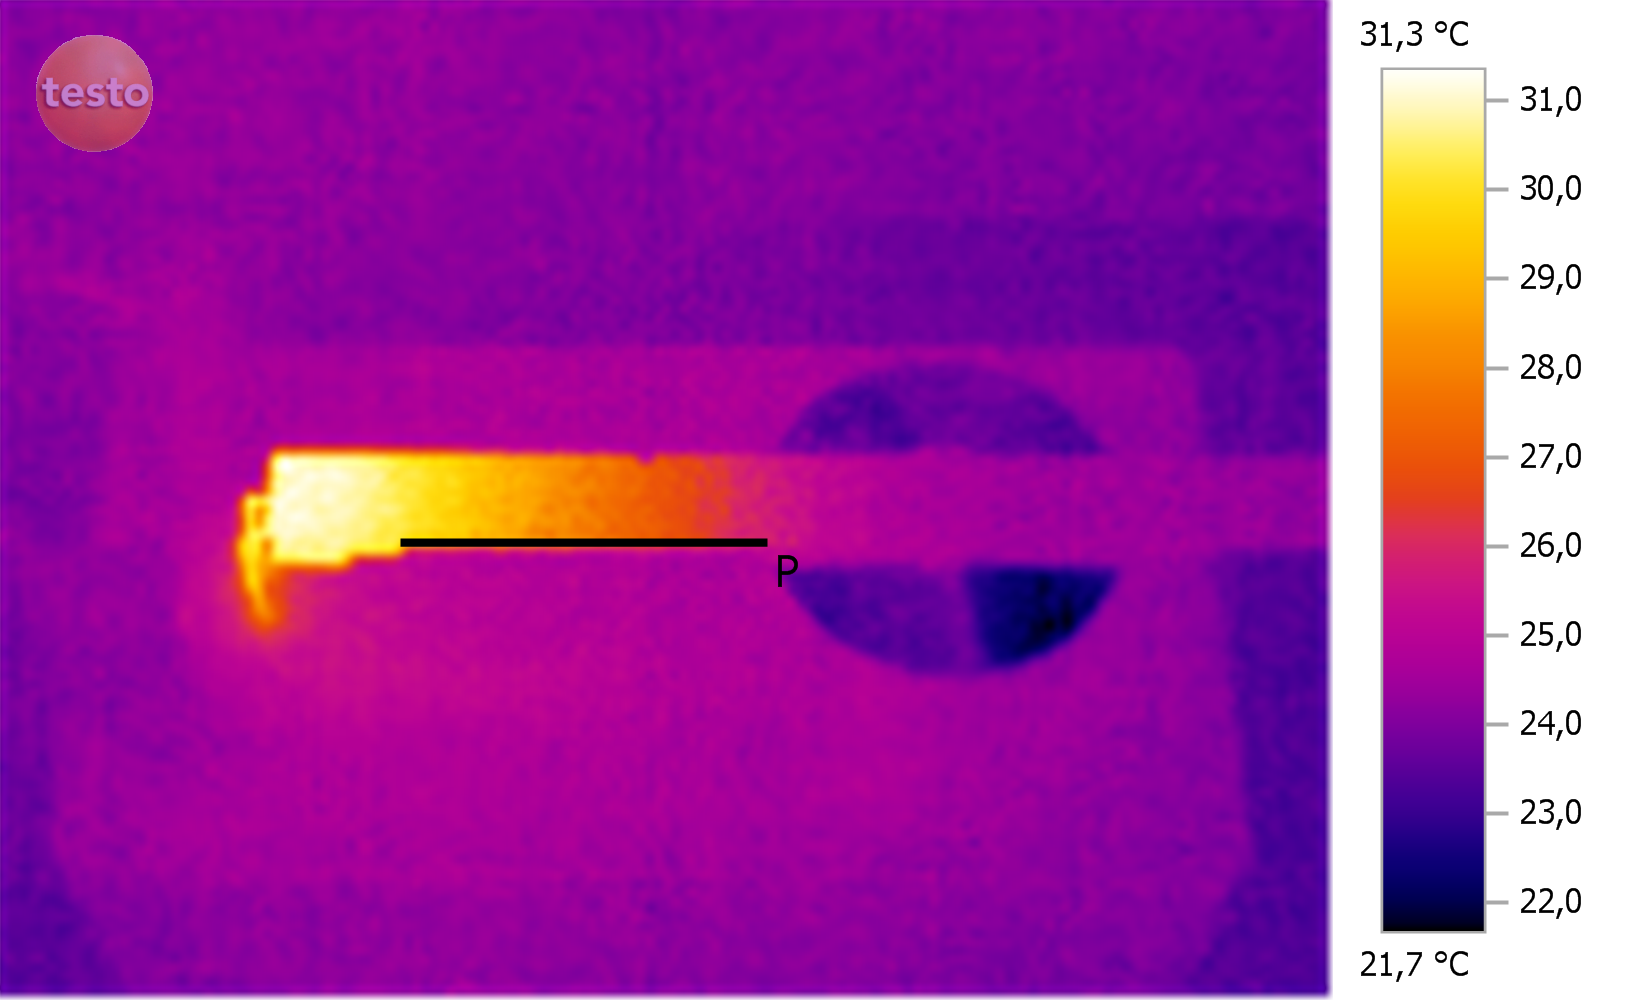
\includegraphics[scale=0.12]{./BilderCorrect/Versuch_1_stationaer_roh.png}
	\caption{Stationärer Temperaturverlauf in Aluminium}
	\label{fig:stat_verlauf}
\end{figure}

\end{multicols}
\begin{figure}[H]
	\centering
	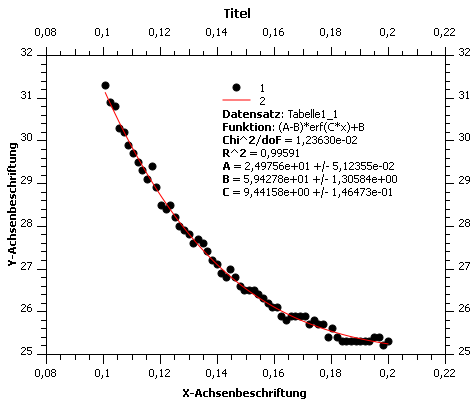
\includegraphics[scale=7]{./BilderCorrect/nicht_stationaer_temp_verlauf.png}
	\caption{Nicht stationärer Temperaturverlauf in Aluminium }
	\label{fig:nicht_stat_verlauf}
\end{figure}
\begin{multicols}{2}

\textbf{Nicht stationärer Temperaturverlauf}
\begin{figure}[H]
	\centering
	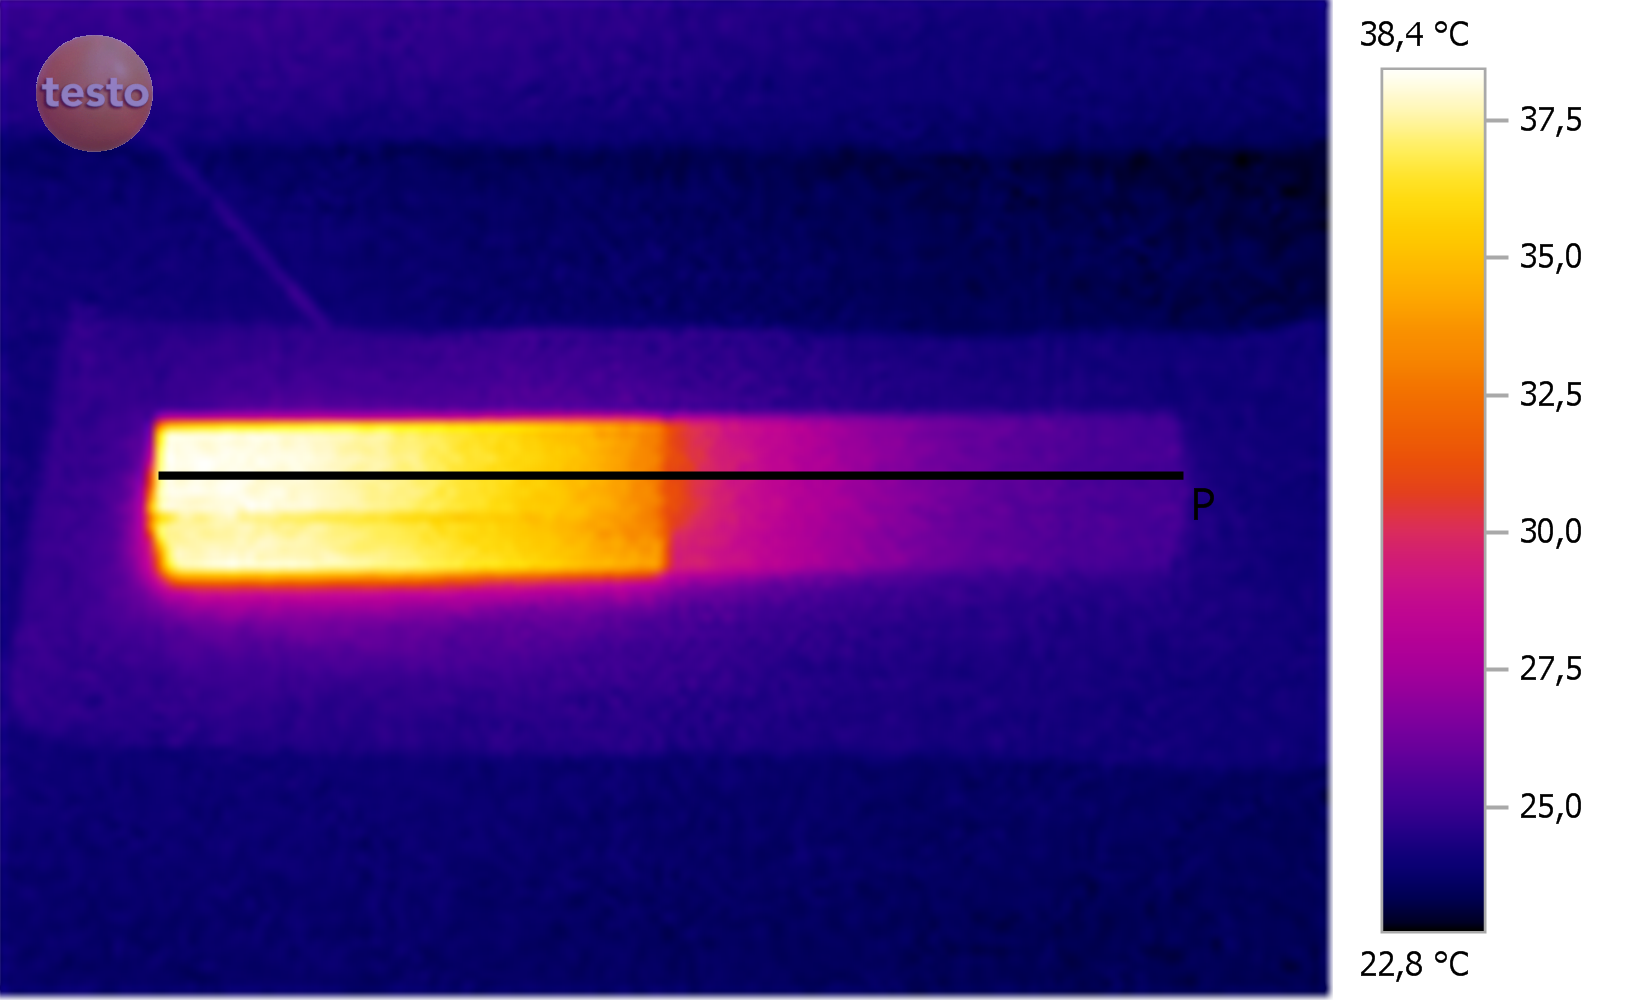
\includegraphics[scale=0.12]{./BilderCorrect/Versuch_1_gradient_60.png}
	\caption{Nicht stationärer Temperaturverlauf in Eisen}
	\label{fig:nicht_stat_verlauf}
\end{figure}

$$\lambda = ( \pm )$$

Die Rohdaten sind unter [2] auffindbar.

\subsection{Diskussion}
Ein nicht klar hervorgegangener Sachverhalt der eine ordentliche Auswertung erst möglich macht, ist das die Wärmeleitpaste nur zur Verminderung des Luftpolsters zwischen den Stäben dient. Beim ersten Versuchsdurchlauf wurde zu viel Paste verwendet und daher ein steiler Temperaturabfall festgestellt (Isolator Wirkung).\\


%%%%%%%%%%%%%%%%%%%%%%%%%%%%%%%%%%%%%%%%%%%%%%%%
%%%%%%%%%%%%%%%%%%%%%%%%%%%%%%%%%%%%%%%%%%%%%%%%

\section{Wärmeleitfähigkeit von Wärmeisolatoren}
In diesem Experiment wird die Wärmeleitfähigkeit eines nicht genau bekannten, isolierenden, Materials bestimmt (Rigips/ Gipskarton).

\subsection{Grundlagen}
Zunächst wird ein Wärmeisolator betrachtet zwischen 2 verschiedenen Wärmereservoirs $T_{w1}$ und $T_{w2}$. Wird eine Seite konstant beheizt, stellt sich nach einiger Zeit ein Gleichgewicht ein, das System befindet sich in einem stationären Zustand.\\
Das bedeutet, dass Wärmeenergie gleichmäßig von der beheizten zur nicht beheizten Seite fließt, also der Wärmestrom $\Phi$ konstant ist:
$$\Phi=\frac{dQ}{dt}=\lambda \cdot A \cdot \frac{(T_{w1}-T_{w2})}{d}$$
mit Q... Wärmestrom\\
A... Querschnittsfläche des Isolators\\
d... Dicke des Isolators\\
$\lambda$... Wärmeleitkoeffizient\\
Die Wärmestromdichte ist gegeben als\\
$q=\Phi/A$\\
Wie Wärmestrom und Wärmestromdichte, wird auch ein Wärmewiderstand $R_{\lambda}$ in Analogie zur Elektrizität definiert als:
$$R_{\lambda}=\frac{1}{\lambda}\cdot \frac{d}{A} $$
der schlüssig mit zunehmender Dicke größer wird, mit zunehmendem Wärmeleitkoeffizienten oder Fläche des Isolators, kleiner.\\
Weiters sind die Wärmeübergangskoeffizienten $\alpha$ von Bedeutung, die den Wärmeübergang von den Wänden des Isolators zur angrenzenden Luft beschreiben. Aufgrund seiner Oberflächenbeschaffenheit entstehen Konvektionsströme in den Grenzschichten:
$$\Phi = \alpha_1 \cdot A \cdot (T1-T_{w1}) = \alpha_2 \cdot A \cdot (T_{w2}-T_2) $$

\noindent In diesem Experiment wird ein \emph{Zweiplattenmessverfahren} angewendet: Es werden zwei Isolatoren direkt aneinander zwischen die beiden Wärmereservoirs gebracht, wobei der Wärmeleitkoeffizient des einen bekannt ist (hier Polysterol, $\lambda = 0.16 \frac{W}{m \cdot K}\pm 0.5\%$).\\
Da im stationären Zustand der Wärmestrom $\Phi$ in allen Schichten (näherungsweise) gleich ist, ergibt sich:
$$\Phi=\lambda_a \cdot A_a \cdot \frac{(T_{w1}-T_{w2})}{d_a}=\lambda_b \cdot A_b \cdot \frac{(T_{w2}-T_{w3})}{d_b}$$
$$\Phi = \alpha_a \cdot A_a \cdot (T1-T_{w1}) = \alpha_b \cdot A_b \cdot (T_{w3}-T_2) $$


\subsection{Versuchsaufbau}
In einer isolierten Wärmekammer wird das Zweiplattensystem aufgebaut. Dieser verfügt an mehreren Stellen über Öffnungen, durch die jeweils ein Thermoelement, zur Messung der Temperatur, eingebracht werden kann:\\
Von unten wird die Wärmekammer (hier mit einigen ohmschen Widerständen) beheizt. Das erste Thermoelement misst $T_1$.
Danach werden die bekannte Eichplatte sowie die Probe aufgelegt. Beide werden zur besseren Wärmeübertragung von Metallplatten umschlossen, die jeweils an der Außenseite schwarz und rau lackiert sind und nach innen reflektieren.\\
In den beiden Platten sind Rillen eingeschnitten, die zu Metallkontakten führen. Hier können die Thermosonden, ohne eine Luftschicht zwischen den Platten zu erzeugen, die Temperatur nahe der Mitte der jeweiligen Platte messen.\\

\noindent  $T_1$... Temperatur der beheizten Luft\\
$T_{w1}$... Außentemperatur an der Eichplatte\\
$T_{w2}$... Temperatur zwischen den Platten\\
$T_{w3}$... Außentemperatur an der Probe\\
$T_2$... Temperatur außen\\

\noindent Das System wird mit einer Steinplatte abgeschlossen.\\
Es dauert etwas mehr als 2 Stunden, bis der Wärmestrom annähernd konstant bleibt. Die Temperaturen werden während der Heizphase protokolliert.\\

\noindent Die Temperaturmessung mit den Termoelementen wird mit dem Fluke 179 Voltmeter durchgeführt und nutzt den Seebeck-Effekt:\\
2 Drähte aus verschiedenen Metallen bzw. Legierungen sind miteinander verlötet. Bei unterschiedlichen Temperaturen, entstehen aufgrund der unterschiedlichen Fermi-Energien beider Drähte Kontaktspannungen. Diese werden mit dem Voltmeter gemessen (und daraus automatisch die Temperatur berechnet).

\end{multicols}
\subsection{Resultate}
\begin{figure}[H]
	\centering
	\pgfplotstabletypeset[
			columns={T1, Tw1, Tw2, Tw3, t},
			col sep=&,
			columns/T1/.style={precision=1, zerofill, column name=\makecell{$T1 - Heizg.$\\$(\pm 0.1)[^\circ C]$} }, 
			columns/Tw1/.style={column name=\makecell{$Tw1$\\$(\pm 0.1)[^\circ C]$}, precision=1},
			columns/Tw2/.style={column name=\makecell{$Tw2$\\$(\pm 0.1)[^\circ C]$}, precision=1},
			columns/Tw3/.style={column name=\makecell{$Tw3$\\$(\pm 0.1)[^\circ C]$}, precision=1},
			columns/t/.style={column name=\makecell{Zeit $t$\\$(\pm 1)[min]$}, precision=0},
			every head row/.style={before row=\hline,after row=\hline\hline},
			every last row/.style={after row=\hline},
			every first column/.style={column type/.add={|}{} },
			every last column/.style={column type/.add={}{|} }
			]{
			T1 & Tw1 & Tw2 & Tw3 & t
			58.5 & 39.0 & 31.8 & 28.3 & 30
			64.2 & 43.6 & 26.5 & 31.8 & 60
			67.7 & 47.1 & 38.9 & 34.4 & 90
			69.5 & 49.3 & 40.9 & 36.0 & 120
			72.4 & 50.8 & 43.3 & 37.2 & 150
			
			}
	\caption{Protokoll der Temperaturen im Aufbau, wärend der Aufheizphase}
	\label{tab:temp-prot}
\end{figure}
\begin{multicols}{2}

\noindent \textbf{Messwerte:}\\
\noindent Eichplatte (Polystrol):\\
$\lambda_{Eich} = 0.16 \frac{W}{m \cdot K}\pm 0.5\%$\\
$A_{Eich}=(22.643 \pm 0.011)\times 10^{-3}m^3 $\\
$d_{Eich}=(10.00 \pm 0.05)\times 10^{-3}m$\\

\noindent Probe (Gipskarton):\\
$A_{Probe}=(22.665 \pm 0.011)\times 10^{-3}m^3$\\
$d_{Probe}=(10.00 \pm 0.05)\times 10^{-3}m$\\

\noindent \textbf{Aufgabe 1:}\\
Wärmestrom:\\
$\Phi = (2.717 \pm 0.057)W$\\
Wärmestromdichte:\\
$q=(120.0 \pm 2.5)W/m^2$\\

\noindent \textbf{Aufgabe 2:}\\
Wärmeleitkoeffizient:\\
$\lambda_{Probe}=(0.1965 \pm 0.0065)\frac{W}{m \cdot K}$\\
Wärmeübergangskoeffizienten:\\
$\alpha_1=(5.56 \pm 0.13 )\frac{W}{m^2 \cdot K}$\\
%$\alpha_2=(5.56 \pm 0.13 )\frac{W}{m^2 \cdot K}$\\
%%T2 nicht gemessen.. wert besorgen von anderer gruppe.. fertig rechnen
%% Zugeben, dassmas verschissen haben

\subsection{Diskussion}
Der ermittelte Wärmeleitkoeffizient $\lambda_{Probe}$ liegt im erwarteten Bereich. Da jedoch nicht genau bekannt ist, welcher Gipskarton verwendet wurde (die Literaturwerte variieren leicht, je nach Variante und Norm), lässt sich die Methode allein durch den Vergleich nicht bewerten.\\
Jedenfalls sind im Messaufbau einige Ungenauigkeiten enthalten:\\
Die Rillen für die Thermoelemente erzeugen Luftpolster, die Kontaktscheiben sitzen nicht ganz in der Mitte der Platten.\\
Außerdem können beim Messen der Dicke der Probeplatte die zahlreichen Vertiefungen in der Oberfläche, nicht gut berücksichtigt werden.\\
Desweiteren ist auch fraglich, ob sich, im Rahmen der Praktikumsdauer, bereits wirklich stabile Verhältnisse eingestellt haben.\\
Die Messverfahren selbst (Thermoelement und Schiebelehre) sind jedoch sehr genau und erzeugen dementsprechend kleine Unsicherheiten. In den Ergebnissen wurden die angesprochenen möglichen Fehler also nicht (durch eine gröbere Abschätzung) berücksichtigt. Dies bedürfte einer gesonderten Untersuchung des Temperatur-Gleichgewichts (mehr Zeit), und der der Effekte, die durch die Oberflächen der Probe und Eichplatte entstehen.\\


\section{Quellen}
$[1]$ Anleitung, \url{http://www.univie.ac.at/anfpra/neu1/ps/ps10/PS10.pdf}\\
$[2]$ Rohdaten, \url{https://github.com/blackandcold/Protocols-SS2014-P2/tree/master/PS_10/BilderCorrect}\\

\end{multicols}
\end{document}